\newpage
\subsection{Inclination Variations}
This series of tests involved evaluating the effect of uniformly changing the inclination of each satellite from the reference case specified in Table \ref{tab:satRefCase} on the performance metrics outlined in Section \ref{sec:perfMetrics}.
\subsubsection{Input Variables}
From the reference case specified in Table \ref{tab:satRefCase}, the inclinations of each satellite were varied between 30 degrees and 90 degrees in 10 degree steps according to Table \ref{tab:inclinationParams}.

\begin{table}[H]
  \centering
  \caption{Inclination variations used}
    \begin{tabular}{p{2.5cm}r}
    \toprule
    Case Number & Inclination (degrees) \\
    \midrule
    1     & 30    \\
    2     & 40  \\
    3     & 60   \\
    4     & 70 	\\
    5     & 80    \\
    6     & 90   \\
    \bottomrule
    \end{tabular}%
  \label{tab:inclinationParams}%
\end{table}%
All other orbital parameters remained constant as per Table \ref{tab:satRefCase}. The ground tracks of the constellation inclined at 30 degrees, 60 degrees and 90 degrees is shown in Figures \ref{fig:12sat_30deg}, \ref{fig:12sat_60deg} and \ref{fig:12sat_90deg} respectively.
\begin{figure}[H]
	
	\begin{subfigure}[b]{\textwidth}
	\centering
	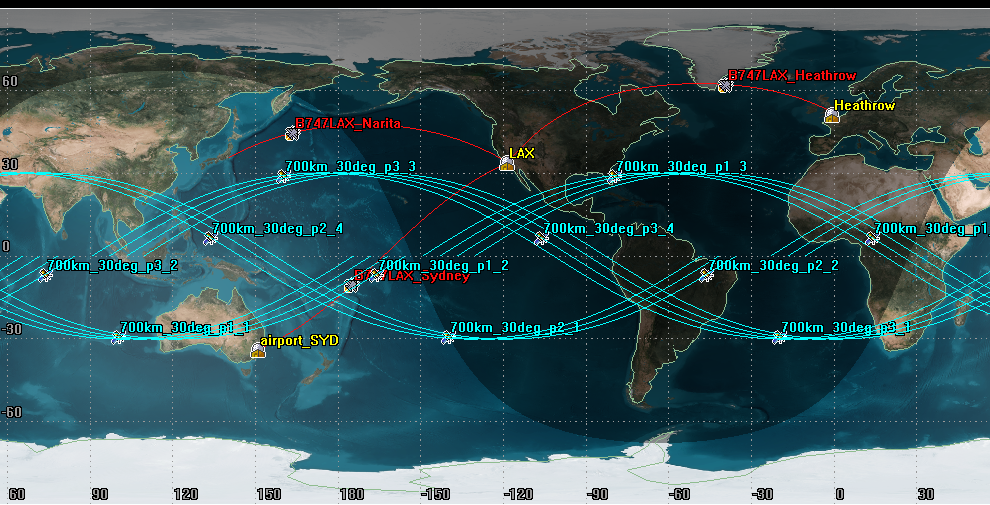
\includegraphics[scale = 0.45]{Pictures/12sat_30deg.png}
	
	\caption{Ground track of satellites inclined at 30 deg (Case 1)}
	\label{fig:12sat_30deg}
	\end{subfigure}
	
	\begin{subfigure}[b]{\textwidth}
	\centering
	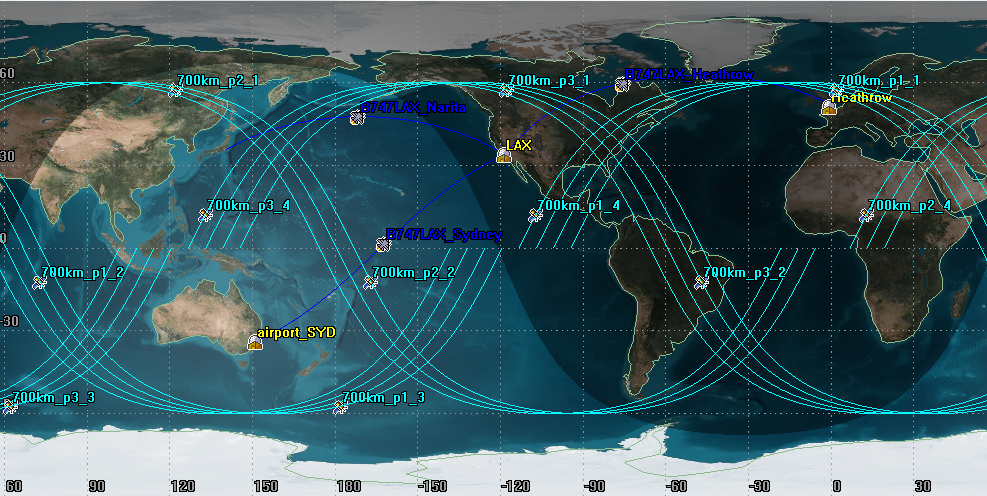
\includegraphics[scale = 0.45]{Pictures/12sat_60deg.png}
	
	\caption{Ground track of satellites inclined at 60 deg (Case 3)}
	\label{fig:12sat_60deg}
	\end{subfigure}
		
	
	\begin{subfigure}[b]{\textwidth}
	\centering
	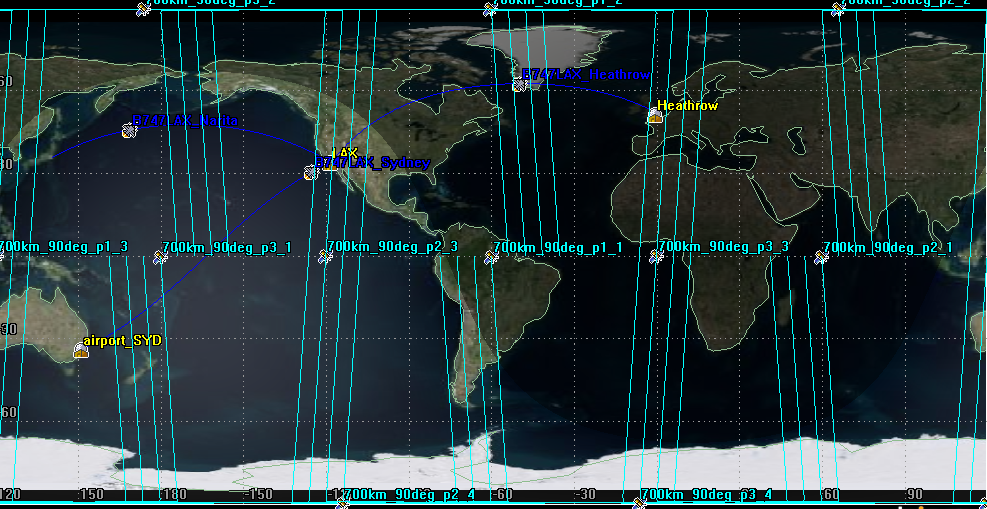
\includegraphics[scale = 0.45]{Pictures/12sat_90deg.png}
	
	\caption{Ground track of satellites inclined at 90 deg (Case 6)}
	\label{fig:12sat_90deg}
	\end{subfigure}
	
	\caption{Ground tracks of constellations inclined between 30 degrees and 90 degrees}
\end{figure} 

\subsubsection{Trends}
The results for inclination variations against the resulting coverage gap fractions, maximum gap period and minimum received signal power are shown in Figures \ref{fig:InclinationVsCovGap12sat}, \ref{fig:InclinationVsMaxGap12sat} and \ref{fig:InclinationVsRxPower12sat} respectively. Each parameter behaved differently for each flight.
\begin{figure}[htbp]
	\centering
	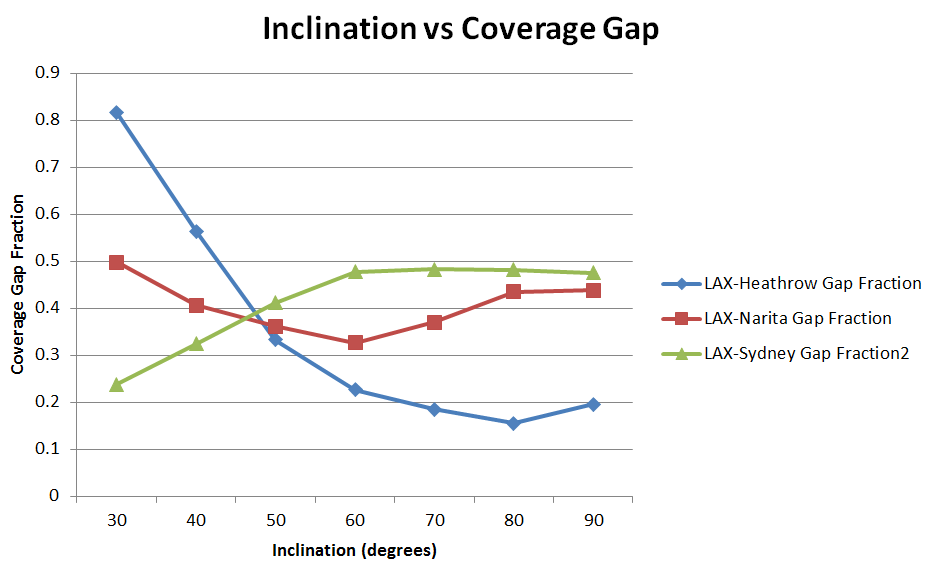
\includegraphics[scale = 0.6]{Pictures/InclinationVsCovGap12sat.png}
	
	\caption{Coverage gap (as a fraction of total analysis time) as effected by inclination  variations. Lower is better}
	\label{fig:InclinationVsCovGap12sat}
\end{figure} 


\begin{figure}[htbp]
	\centering
	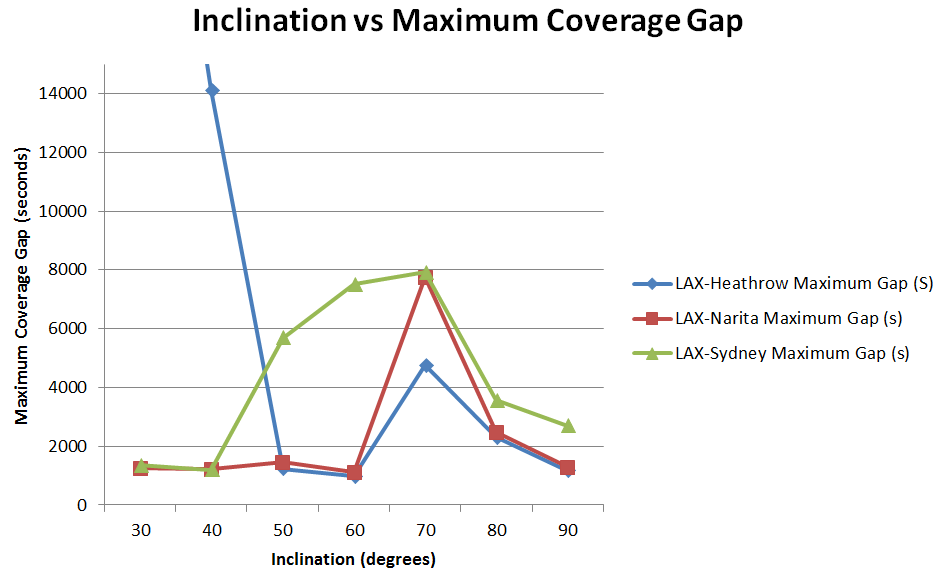
\includegraphics[scale = 0.6]{Pictures/InclinationVsMaxGap12sat.png}
	
	\caption{Maximum coverage gap as affected by altitude variations. Lower is better.}
	\label{fig:InclinationVsMaxGap12sat}
\end{figure} 

\begin{figure}[htbp]
	\centering
	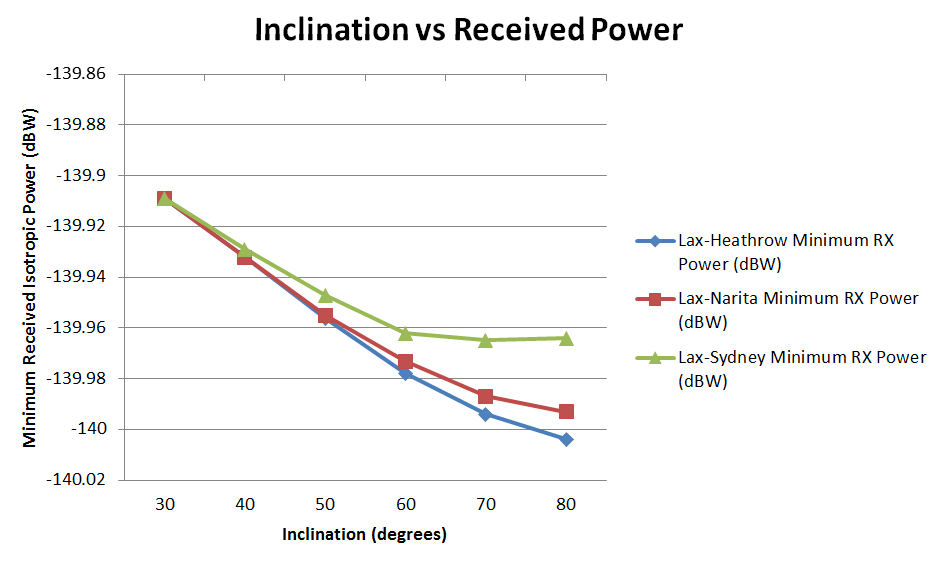
\includegraphics[scale = 0.6]{Pictures/InclinationVsRxPower12sat.png}
	
	\caption{Minimum received isotropic power as affected by inclination variations. Higher is better.}
	\label{fig:InclinationVsRxPower12sat}
\end{figure}
\subsubsection{Discussion}
At lower inclinations, the ground tracks of the satellite have a significant amount of coincidence with the flight path between LAX and Sydney, as seen in Figure \ref{fig:12sat_30deg}. This results in the LAX-Sydney flight path having an optimised maximum coverage time and coverage fraction at 30 degrees inclination as can be seen on Figures \ref{fig:InclinationVsCovGap12sat} and \ref{fig:InclinationVsMaxGap12sat}. Increasing inclinations resulted in a higher coverage gap ratio, before settling at 60 degrees and remaining constant through to 90 degrees.

The relatively high inclination of the LAX-Heathrow flight path resulted in poor coverage performance with the constellation at low inclinations. At low inclinations there were few opportunities for line of sight to be established between the LAX-Heathrow flight, with access periods only occurring when satellites reached high latitudes at the same time as the flight was at a low latitude. The resulting maximum gap (not shown in Figure \ref{fig:InclinationVsMaxGap12sat} for scale purposes) was 29 866 seconds (8 hours and 18 minutes) - more than half the duration of the flight. The aggregate result also yielded a poor coverage gap fraction performance below 50 degrees, as seen in Figure \ref{fig:InclinationVsCovGap12sat}. The effect sharply decreased with higher inclinations, with coverage gaps lowering to an acceptable level after 50 degrees.

All flight paths observed a spike in maximum coverage gap time with satellites inclined at 70 degrees, as seen in Figure \ref{fig:InclinationVsMaxGap12sat}. This occurred due to the geometry of the constellation and the effect of the Earth's rotation under the constellation. Figure \ref{fig:70_deg_precess_1_edited} shows that the effective width between the two orbital planes of the satellite is quite high, creating an effective radio `dead zone' in which the pictured plane cannot access a satellite. Although the plane continues to travel out of the `dead zone', the rotation of the Earth underneath the constellation moves the position of the plane back into the `dead zone', as demonstrated in  Figure \ref{fig:70_deg_precess_2_edited}. At inclinations of 80 degrees and 90 degrees this effect is mediated by the changing geometry and intersections between satellite ground tracks and flight paths, resulting in more acceptable coverage gaps.

There is relatively little change in the minimum received isotropic powers, with values ranging between -139.9 dBW and -140.02 dBW as seen in Figure \ref{fig:InclinationVsRxPower12sat}. The observed trend occurs due to the satellite having a higher chance of being `directly overhead' with higher inclinations, resulting in a shorted free-path propagation distance for the ADS-B signal. However this effect was quite small, only resulting in a net change of 0.12 dBW across the experimented range.

\begin{figure}[htpb]
	\centering
	\begin{subfigure}[b]{0.6\textwidth}
	
	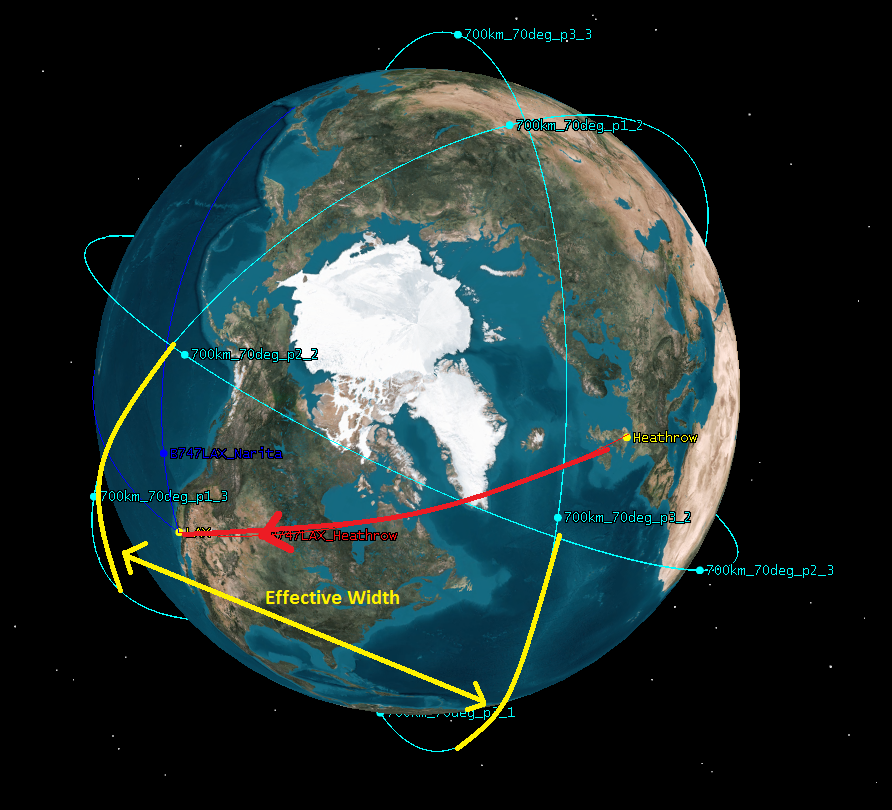
\includegraphics[width=\textwidth]{Pictures/70_deg_precess_1_edited.png}
	
	\caption{Flight initially in `dead zone' of no ADS-B access between planes}
	\label{fig:70_deg_precess_1_edited}
	\end{subfigure}
	
	\begin{subfigure}[b]{0.6\textwidth}
	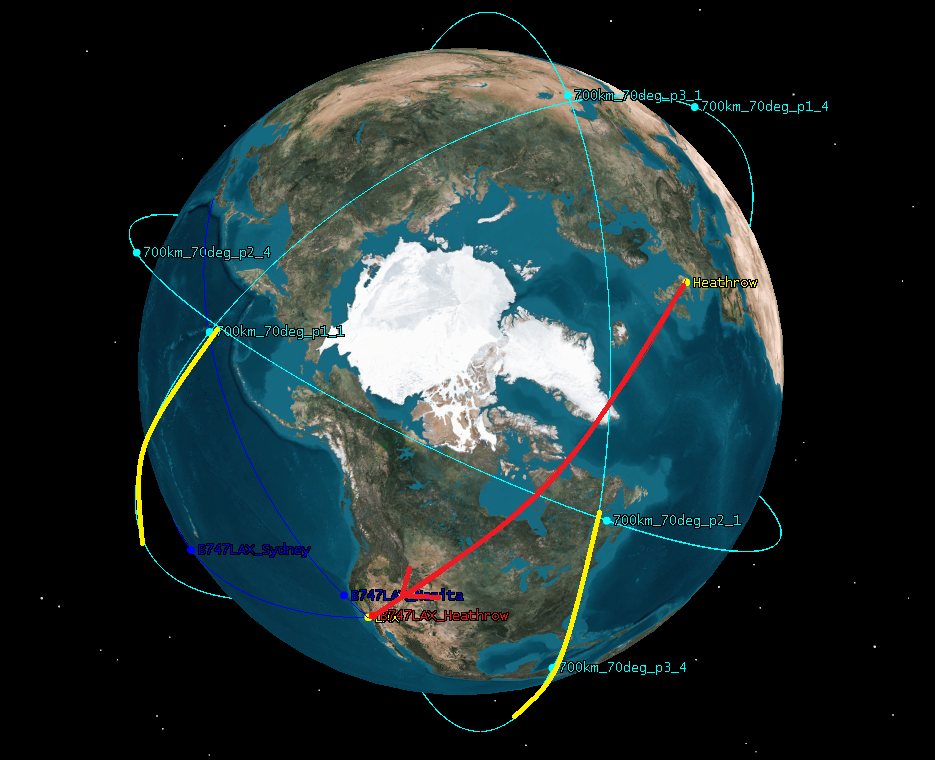
\includegraphics[width=\textwidth]{Pictures/70_deg_precess_2_edited.png}
	
	
	\caption{Rotation of Earth eastward keeps the flight in the `dead zone' for an extended period of time}
	\label{fig:70_deg_precess_2_edited}
	\end{subfigure}
		
	
	\caption{Flight in `dead zone' between satellite planes, inclined at 70 degrees. View from North Pole}
\end{figure} 